A proton (charge 1) and an electron (charge 2) move to the right side by side, as shown. Consider only the magnetic forces between them (the electric force between them is larger, but it is not asked here).

\begin{center}
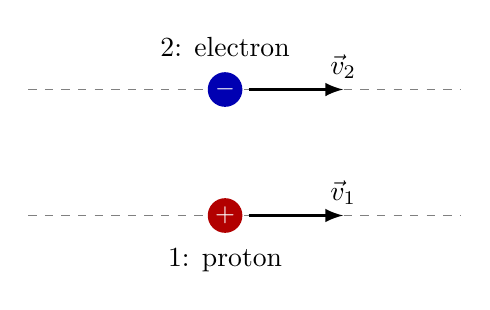
\begin{tikzpicture}[>=latex]
 \draw[dashed, gray] (-2.5,0) -- (3,0);
 \draw[dashed, gray] (-2.5,1.6) -- (3,1.6);
 \fill[red!70!black] (0,0) circle (0.22); \node[white] at (0,0) {\small $+$};
 \node[below] at (0,-0.3) {1: proton};
 \draw[->, very thick] (0.3,0) -- (1.5,0) node[above] {$\vec v_1$};
 \fill[blue!70!black] (0,1.6) circle (0.22); \node[white] at (0,1.6) {\small $-$};
 \node[above] at (0,1.9) {2: electron};
 \draw[->, very thick] (0.3,1.6) -- (1.5,1.6) node[above] {$\vec v_2$};
\end{tikzpicture}
\end{center}

\begin{abcliste}
\abc In which direction does the magnetic field of charge 1 point at the place of charge 2?
\abc In which direction does the magnetic force on charge 2 point?
\abc Do the magnetic forces pull the two particles together or push them apart?
\end{abcliste}
